%%%%%%%%%%%%%%%%%%%%%%%%%%%%%%%%%%%%%%%%%%%%%%
%                insertmeeting
% 1) Title (something creative & funny?)
% 2) Date (MM/DD/YYYY)
% 3) Location (ex. Hagerty High School)
% 4) People/Committees Present 
% 5) Picture 
% 6) Start Time & Stop Time (ex. 12:30AM to 4:30PM)
%%%%%%%%%%%%%%%%%%%%%%%%%%%%%%%%%%%%%%%%%%%%%%
\insertmeeting 
	{Introducing Cram Week} 
	{02/27/23} 
	{Hagerty High School}
	{Karissa, Laura, Tyler, Samantha, Nathan, Robert, Jensen, Anouska, Mohana, Ritam, Jorge}
	{Images/RobotPics/robot.jpg}
	{2:30 - 5:00}
	
\hhscommittee{General}
\noindent\hfil\rule{\textwidth}{.4pt}\hfil
\subsubsection*{Goals}
\begin{itemize}
    \item Adjust and practice our States Presentation
    \item Review tasks for States preparations
\end{itemize} 

\noindent\hfil\rule{\textwidth}{.4pt}\hfil

\subsubsection*{Accomplishments}
On Monday, we began our final preparations for the States competition coming up this Saturday, primarily focussing on Presentation, which is Tuesday. We started by discussing all the non-robot tasks that we needed to complete this week, as well as decided who would take the lead on each task. Several members made a list of supplies to order for our pit at States. At 3:15 and 4:00, we did run-throughs of tomorrow’s presentation in order to work out the kinks and know our parts well enough to present smoothly and within the time frame. At 4:30, we participated in a Zoom meeting with Mr. ___, who listened to our presentation and gave us some insightful advice.

 
%\begin{figure}[htp]
%\centering
%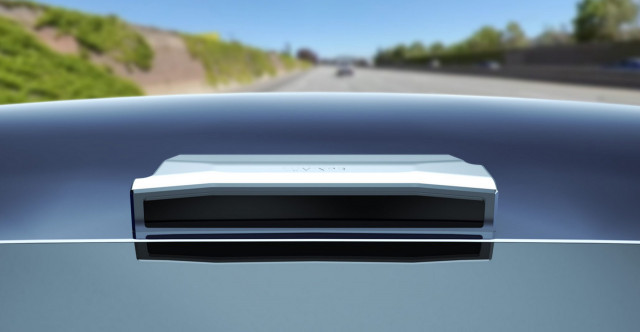
\includegraphics[width=0.95\textwidth, angle=0]{Meetings/February/02-07-23/luminar-iris-roof-mounted-lidar_100767931_m.jpg}
%\caption{Luminar's lidar technology for self-driving cars}
%\label{fig:pic1}
%\end{figure}


\whatsnext{
\begin{itemize}
    \item Make buttons for State Competition
    \item Finalize Engineering Notebook
    \item Order supplies for State Competion Pit and team gifts
    \item Design and print posters
\end{itemize} 
}